\chapter{DishBrain}
\chaptermark{DishBrain}
\label{sec:dishbrain}

\section{Uma rede na placa joga tênis}

DishBrain é o nome que os autores deram à bancada em que uma cultura de neurônios vivos, cultivada sobre um chip com eletrodos, joga um tênis simplificado com uma só raquete~\cite{Kagan2022}. É o experimento mais discutido com uma máquina de neurônios vivos (um panorama dessas máquinas está no capítulo~\ref{sec:livingmachine}), e para o nosso livro ele é especialmente conveniente. Aqui a pequena rede está acessível por inteiro: cada entrada é definida pelo experimentador, cada saída é registrada. Todas as perguntas dos capítulos anteriores (como o sinal é codificado, quem ensina, o que a sonda vê) podem ser feitas a uma rede que não tem olhos, nem músculos, nem neurônios \nt{DOPA}. Vamos analisar o experimento como um engenheiro analisa a bancada de outra pessoa: esquema, entrada, saída, professor, resultado, controvérsias.

\section{A bancada}

Os neurônios vêm do córtex de embriões de camundongo, cerca de $800\,000$ células por chip, ou são cultivados a partir de células-tronco humanas, cerca de um milhão por chip. Durante algumas semanas eles crescem no chip, entrelaçam-se e começam a produzir sozinhos disparos e rajadas. Numa área de $8$~mm$^2$ sob eles há $26\,000$ eletrodos de platina; até $1024$ deles podem ser registrados ao mesmo tempo, e a estimulação, na prática, se faz por oito.

Em torno da cultura fecha-se uma malha (fig.~\ref{fig:dishloop}). O computador simula o jogo: a bola voa, bate nas paredes, a raquete se move para cima e para baixo. A posição da bola é convertida em corrente em oito eletrodos ``sensoriais''. Os disparos de duas regiões ``motoras'' são contados em janelas de $10\ms$ e movem a raquete. Depois de cada acerto ou erro, a cultura recebe mais um estímulo: a realimentação. As janelas de $10\ms$ são o ciclo do computador da bancada, não da cultura: a própria rede continua funcionando de forma assíncrona, como todas as redes deste livro.

\begin{figure}[t]
\centering
\begin{tikzpicture}[>=Stealth,
  blk/.style={draw,very thick,rounded corners=3pt,align=center,font=\small,minimum height=1.2cm},
  lab/.style={font=\scriptsize,align=center}]
\node[blk,fill=blue!6,text width=3.4cm] (C) at (0,0) {cultura no chip\\\scriptsize $\sim10^6$ neurônios, $26\,000$ eletrodos};
\node[blk,fill=orange!10,text width=3.0cm] (G) at (7.2,0) {computador:\\jogo de tênis};
\draw[->,very thick,blue!60!black] (G.north west) to[bend right=25] node[lab,above] {bola: \emph{lugar} = qual dos 8 eletrodos,\\\emph{frequência} = 4--40 disparos/s} (C.north east);
\draw[->,very thick,red!70!black] (C.south east) to[bend right=25] node[lab,below] {raquete: contagem de disparos\\das regiões ``sobe'' e ``desce'' em $10\ms$} (G.south west);
\draw[->,thick,densely dashed,green!45!black] (G.east) -- ++(0.9,0) |- ++(0,-2.6) -| node[lab,pos=0.25,below] {acerto: estímulo previsível; erro: imprevisível} (C.south);
\end{tikzpicture}
\caption{A malha do DishBrain. Seta azul: entrada; a posição da bola é codificada por código de lugar e código de taxa (capítulo~\ref{sec:code}). Vermelha: saída; a diferença entre as contagens das duas regiões move a raquete. Verde tracejada: realimentação depois de cada rali, o único ``professor'' da bancada.}
\label{fig:dishloop}
\end{figure}

\section{Entrada e saída}

A \emph{entrada} usa ao mesmo tempo dois códigos do capítulo~\ref{sec:code}. Qual dos oito eletrodos é estimulado diz a que altura está a bola: é um código de lugar, como nos sensores do capítulo~\ref{sec:sensors}. A frequência dos pulsos de estimulação diz a que distância está a bola: $4$ por segundo quando ela está junto à parede do fundo, e linearmente mais, até $40$ por segundo, quando está junto à parede da raquete. É um código de taxa; a amplitude dos pulsos da bola é de $75$~mV. A cultura não ``conhece'' nenhum desses códigos de antemão: o código foi definido pelo experimentador, e a rede tem de aprender a lê-lo.

A \emph{saída} é lida como nas interfaces do capítulo~\ref{sec:debugging}. Os disparos de uma região motora empurram a raquete para cima, os da outra, para baixo; na forma mais simples, a cada janela
\begin{empheq}[box=\keybox]{equation}
\Delta p \;=\; c\,\bigl(n_\uparrow - n_\downarrow\bigr),
\label{eq:dishreadout}
\end{empheq}
em que $n_\uparrow$, $n_\downarrow$ são os números de disparos das duas regiões em $10\ms$, e $c$ é um coeficiente da bancada. É o código de dois fios do capítulo~\ref{sec:glutcomputer}: o sentido do movimento não depende de o sinal elétrico ser positivo ou negativo, e sim de qual dos dois fios fala mais alto.

Vejamos o ruído dessa saída. Se uma região produz ao todo $R$ disparos por segundo, numa janela $T=10\ms$ há em média $RT$ deles, e por~\eqref{eq:rateerror} a dispersão relativa é $1/\sqrt{RT}$. Com $R=1000$ disparos por segundo, isso dá cerca de $30$ por cento em cada janela; com $R=100$, mais de cem. A raquete inevitavelmente treme, e a rede só pode aprender de um jeito: deslocando a diferença \emph{média} das contagens para o lado certo. São as mesmas leis que limitam qualquer interface do capítulo~\ref{sec:debugging}, só que agora dos dois lados da malha.

\section{Um professor sem dopamina}

O mais interessante na bancada é o professor. Numa cultura de neurônios do córtex não há neurônios \nt{DOPA}, e a bancada não envia nenhum sinal de ``melhor do que o esperado''. A realimentação é outra. Se a rede rebateu a bola, os oito eletrodos sensoriais recebem ao mesmo tempo um estímulo curto e \emph{previsível}: pulsos de $75$~mV, $100$ por segundo durante $0.1\,\text{s}$. Se errou, durante quatro segundos vem um estímulo que os autores chamam de \emph{imprevisível}: pulsos de $150$~mV, $5$ por segundo, em momentos aleatórios e em eletrodos escolhidos ao acaso; depois, quatro segundos de pausa sem estimulação, e a bola parte de novo~\cite{Kagan2022}.

Os autores partiram da hipótese de que a rede age de modo a tornar sua entrada previsível~\cite{Friston2010}. Para um engenheiro o sentido é simples: a cultura tem exatamente um jeito de se livrar de quatro segundos de ruído aleatório, que é rebater a bola. A mesma ideia já apareceu na economia de disparos do capítulo~\ref{sec:code} e na predição do quadro no capítulo~\ref{sec:recognition}.

Mas é preciso mesmo a previsibilidade? Um mecanismo mais grosseiro também é possível. Suponha que o estímulo imprevisível depois de um erro simplesmente \emph{embaralhe} as mudanças recentes na rede, e que o estímulo calmo depois de um acerto não mexa nelas. Descrevamos a configuração da rede por um único vetor $\boldsymbol\psi$, e seja $P_{\text{erro}}(\boldsymbol\psi)$ a probabilidade de a rede errar na configuração $\boldsymbol\psi$. Se os empurrões forem simétricos (de $\boldsymbol\psi$ para $\boldsymbol\psi'$ é tão provável quanto o inverso), no regime estacionário o fluxo de saídas de cada configuração se equilibra com o fluxo de chegadas, e a fração do tempo que a rede passa na configuração $\boldsymbol\psi$ é
\begin{empheq}[box=\keybox]{equation}
\rho(\boldsymbol\psi) \;\propto\; \frac{1}{P_{\text{erro}}(\boldsymbol\psi)} .
\label{eq:dishdensity}
\end{empheq}
Uma configuração que erra dez vezes menos é mantida dez vezes mais. Ninguém diz à rede para que lado mudar os pesos: as boas configurações simplesmente são destruídas com menos frequência.

Verificamos isso num modelo que reduz a cultura a dois números: a raquete chega ao ponto $a\,y+b$ quando a bola chega à altura $y$, e rebate se errar por menos de $0.1$. Depois de um erro, os dois números recebem um empurrão aleatório; depois de um acerto, ficam como estão. A fração de bolas rebatidas em $2000$ ralis subiu de $0.21$ nos primeiros duzentos para $0.38$ nos últimos quinhentos (quarenta ``culturas'', fig.~\ref{fig:dishmodel}). Se o empurrão vier depois de \emph{cada} rali, a realimentação não traz informação, e a fração fica em torno de $0.12$; sem empurrão nenhum, ela fica parada em $0.19$. O experimento na bancada concorda com isso: um aumento significativo dentro da sessão só ocorreu com a realimentação completa. Com silêncio no lugar dos estímulos, a cultura ainda assim jogava melhor no fim da sessão do que sem realimentação, mas com efeito menor~\cite{Kagan2022}; note que também nessa condição um erro é seguido de uma pausa longa, e um acerto, de uma curta, de modo que a diferença entre os desfechos não desaparece por completo.

\begin{figure}[t]
\centering
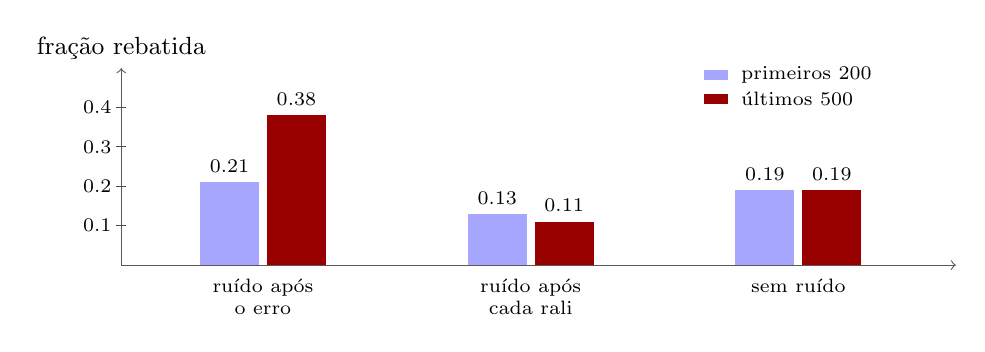
\begin{tikzpicture}[x=1cm,y=5cm]
\draw[->,gray!70!black] (0,0) -- (10.6,0);
\draw[->,gray!70!black] (0,0) -- (0,0.5) node[above,font=\small,black] {fração rebatida};
\foreach \v in {0.1,0.2,0.3,0.4}{\draw[gray!60!black] (-0.06,\v) -- (0.06,\v); \node[left,font=\scriptsize] at (0,\v) {\v};}
\foreach \x/\f/\l/\lab in {1.8/0.21/0.38/{ruído após\\o erro},5.2/0.13/0.11/{ruído após\\cada rali},8.6/0.19/0.19/{sem ruído}}{
  \fill[blue!35] (\x-0.8,0) rectangle (\x-0.05,\f);
  \fill[red!60!black] (\x+0.05,0) rectangle (\x+0.8,\l);
  \node[below,font=\scriptsize,align=center] at (\x,-0.01) {\lab};
  \node[above,font=\scriptsize] at (\x-0.425,\f) {\f};
  \node[above,font=\scriptsize] at (\x+0.425,\l) {\l};}
\fill[blue!35] (7.4,0.47) rectangle (7.7,0.495); \node[right,font=\scriptsize] at (7.75,0.482) {primeiros 200};
\fill[red!60!black] (7.4,0.41) rectangle (7.7,0.435); \node[right,font=\scriptsize] at (7.75,0.422) {últimos 500};
\end{tikzpicture}
\caption{O modelo ``embaralhar no erro'' (\texttt{dishbrain\_model.py}): fração de bolas rebatidas no início e no fim de $2000$ ralis, média de quarenta culturas-modelo. Só há aprendizado se o empurrão vier depois do erro, e não do acerto, como no experimento, em que o aumento significativo na sessão só ocorreu com a realimentação completa.}
\label{fig:dishmodel}
\end{figure}

\begin{keyblock}
\begin{proposition}[O professor embaralhador]
\label{prop:dishscramble}
Se o fracasso sacode a rede e o sucesso a deixa em paz, a rede deriva sozinha para configurações que erram menos: o tempo passado numa configuração é inversamente proporcional à probabilidade de fracasso~\eqref{eq:dishdensity}. Para esse aprendizado não são necessários nem um sinal de recompensa, nem o seu sinal algébrico, nem a previsibilidade em si; basta que a realimentação depois do sucesso e depois do fracasso seja diferente. A mudança de comportamento da cultura está medida; qual mecanismo atua na placa, predição da entrada ou embaralhamento, não está estabelecido.
\end{proposition}
\end{keyblock}

Compare com o capítulo~\ref{sec:dofa}. Lá o ruído também servia de busca, mas a dopamina tinha sinal algébrico: o erro $\delta$ dizia para que lado deslocar os pesos, e o passo seguia o gradiente~\eqref{eq:perturbation}. Aqui não há sinal algébrico, só ``manter'' ou ``sacudir''. Essa busca é mais grosseira e mais lenta, mas exige menos da rede: nem neurônios \nt{DOPA}, nem crítico, nem traço estendido por segundos.

\section{O que foi medido e o que se discute}

Cada jogo durava $20$ minutos; comparavam-se os primeiros $5$ minutos com os últimos $15$. Nas culturas com realimentação completa, as sequências de bolas rebatidas ficaram mais longas, e os erros imediatos, mais raros; nos controles sem células, sem jogo e com uma ``raquete'' de computador, nada parecido aconteceu. As culturas de células humanas em média rebatiam por mais tempo que as de camundongo. A melhora é estatisticamente sólida (em nove culturas de camundongo e onze humanas, em mais de cem jogos de cada grupo), mas pequena: a rede não virou um bom jogador, ficou um pouco melhor que o acaso. Ela é sólida dentro da sessão; aprendizado estável de uma sessão para outra ao longo de vários dias os autores não obtiveram~\cite{Kagan2022}. Num trabalho seguinte do mesmo grupo, verificou-se que durante o jogo a atividade da cultura se aproxima do regime \emph{crítico}, a fronteira entre a extinção e a avalanche, aquela mesma vida no limite do capítulo~\ref{sec:gaba}, e quanto mais perto, melhor o jogo~\cite{Habibollahi2023}.

A principal controvérsia não foi causada pelos números, e sim pelas palavras. O título do artigo afirmava que os neurônios na placa ``exibem senciência'' (sentience), e um grupo de pesquisadores objetou: a mudança de comportamento numa malha fechada ainda não é inteligência nem sensação, e as conclusões deveriam ser formuladas com mais modéstia~\cite{Balci2023}. Do ponto de vista de engenharia, há duas questões em aberto, ambas sobre o mecanismo. Primeira: a rede aprende, isto é, seus pesos mudam de forma duradoura, ou a realimentação só desloca seu estado atual? Segunda: é preciso justamente a previsibilidade, ou basta qualquer diferença entre a resposta ao sucesso e ao fracasso, como na proposição~\ref{prop:dishscramble}? Uma bancada em que cada eletrodo é acessível permite responder às duas, e esse talvez seja seu principal valor.

\section{Especificação da bancada: como reproduzi-la}
\label{sec:dishspec}

Abaixo está reunido tudo o que é preciso para montar essa bancada de novo: equipamento, malha, codificação da entrada, leitura da saída, realimentação e protocolo do experimento. Cada parâmetro traz sua fonte. ``Artigo'': o valor foi tirado do texto do trabalho~\cite{Kagan2022}. ``Escolha'': o artigo não o traz, e para reproduzir será preciso defini-lo por conta própria; propomos um valor padrão e dizemos como verificá-lo.

\subsection*{Equipamento e cultura}

\begin{center}
\footnotesize
\setlength{\tabcolsep}{4pt}
\renewcommand{\arraystretch}{1.15}
\begin{tabular}{>{\raggedright}p{4.0cm}>{\raggedright}p{6.9cm}>{\raggedright\arraybackslash}p{1.6cm}}
\toprule
Parâmetro & Valor & Fonte \\
\midrule
chip & matriz MaxOne: $26\,000$ eletrodos de platina numa área de $8$~mm$^2$ & artigo \\
registro & até $1024$ canais simultâneos, $20\,000$ amostras por segundo & artigo \\
estimulação & até $32$ eletrodos tecnicamente, no experimento $8$ independentes & artigo \\
células & córtex de embrião de camundongo; neurônios humanos de células-tronco (dois métodos de cultivo); células HEK293T (não neurônios) como controle & artigo \\
semeadura & cerca de $10^6$ células por chip & artigo \\
idade da cultura no experimento & camundongo: a partir de $\sim10$ dias; humana: $14$--$24$ dias ou $\sim80$ dias, conforme o método de cultivo & artigo \\
\bottomrule
\end{tabular}
\end{center}

\subsection*{Malha e tempo}

A malha funciona em janelas de $10\ms$ ($200$ amostras): em cada janela contam-se os disparos nos eletrodos das regiões motoras, o jogo é atualizado, e sai a estimulação seguinte. O atraso entre um disparo na cultura e o estímulo de resposta é de cerca de $5\ms$. Durante o jogo, o sinal de cada eletrodo passa por um filtro passa-altas Bessel de 2.ª ordem com frequência de corte de $100$~Hz; o módulo do sinal é suavizado por um filtro passa-baixas Bessel de 1.ª ordem de $1$~Hz, e o limiar de disparo é proporcional a esse módulo suavizado. O limiar de seis desvios-padrão do fundo o artigo indica para medições isoladas de atividade, não para o jogo. Para que a estimulação não seja contada como resposta da cultura, todos os sinais são suprimidos quando chegam ao mesmo tempo mais de $15$ pulsos grandes, acima de $75$~mV. Tudo isso é do artigo.

\subsection*{Codificação da bola}

\begin{center}
\footnotesize
\setlength{\tabcolsep}{4pt}
\renewcommand{\arraystretch}{1.15}
\begin{tabular}{>{\raggedright}p{3.4cm}>{\raggedright}p{7.5cm}>{\raggedright\arraybackslash}p{1.6cm}}
\toprule
Parâmetro & Valor & Fonte \\
\midrule
região sensorial & $8$ eletrodos dispostos de modo que eletrodos vizinhos signifiquem posições vizinhas da bola & artigo \\
código de lugar & o número do eletrodo $k=1,\dots,8$ dá a posição da bola em relação ao centro da raquete & artigo \\
qual coordenada & a posição vertical da bola; para reproduzir, em relação à raquete, $k=\lceil 8(y-p+\tfrac12)\rceil$ com $y-p\in[-\tfrac12,\tfrac12]$ & artigo; fórmula: escolha \\
código de taxa & a frequência de estimulação, de $4$ a $40$~disparos/s, codifica a distância até a raquete & artigo \\
sentido da escala & $4$~disparos/s com a bola junto à parede oposta, e linearmente até $40$~disparos/s junto à parede da raquete: $f=4+36\,(1-x/L)$, $x$ é a distância até a parede da raquete, $L$ a largura da quadra & artigo \\
forma do pulso & curto, retangular, bifásico: primeiro a fase positiva, depois a negativa & artigo \\
amplitude & $75$~mV; escolhida para não forçar o disparo de células inibidas & artigo \\
duração das fases & não indicada; usar o ajuste padrão do sistema de estimulação e não mudá-lo durante o experimento & escolha \\
\bottomrule
\end{tabular}
\end{center}

\subsection*{Leitura da raquete}

No artigo há duas regiões motoras: os disparos na primeira movem a raquete para cima, na segunda, para baixo; a contribuição das regiões é ponderada para levar em conta a diferente densidade de células e a diferente atividade~\cite{Kagan2022}. A fórmula exata não é dada. Para reproduzir, usamos a regra~\eqref{eq:dishreadout}, $\Delta p=c\,(n_\uparrow-n_\downarrow)$ a cada janela de $10\ms$, com um peso que iguala as regiões pela atividade média em repouso (escolha): $n_\uparrow$ e $n_\downarrow$ são divididos pela contagem média da respectiva região por janela, medida antes do jogo. O coeficiente $c$ é escolhido de modo que uma diferença de uma contagem média desloque a raquete $1\%$ da altura da quadra por janela (escolha); assim, uma vantagem constante de uma região leva a raquete de um lado a outro da quadra em $1$~s.

A posição das regiões no chip não é dada em coordenadas no texto do artigo; há apenas um esquema. Para reproduzir bastam três grupos de eletrodos disjuntos: os oito sensoriais no centro e um grupo de eletrodos de registro de cada lado, um ``sobe'' e outro ``desce'' (escolha).

\subsection*{O jogo}

As dimensões da quadra, o comprimento da raquete e a velocidade da bola não constam do artigo; diz-se apenas que a bola se move com velocidade constante e é refletida pelas paredes. Para reproduzir (escolha): quadra $1\times1$, raquete na parede direita com comprimento $0.2$ (acerto se $|y-p|<0.1$, como no modelo~\texttt{models/dishbrain\_model.py}), a bola atravessa a quadra em $1$~s. Um erro sem nenhuma bola rebatida no rali conta como ``ace''; um rali com mais de três acertos seguidos, como ``longo'' (artigo).

\subsection*{Realimentação}

\begin{center}
\footnotesize
\setlength{\tabcolsep}{4pt}
\renewcommand{\arraystretch}{1.15}
\begin{tabular}{>{\raggedright}p{2.6cm}>{\raggedright}p{8.3cm}>{\raggedright\arraybackslash}p{1.6cm}}
\toprule
Evento & O que é aplicado & Fonte \\
\midrule
acerto & estímulo previsível: os $8$ eletrodos sensoriais ao mesmo tempo, $75$~mV, $100$~disparos/s, $100\ms$; a estimulação normal da bola é interrompida durante esse tempo & artigo \\
erro & estímulo imprevisível: $150$~mV, $5$~disparos/s, $4$~s, em momentos aleatórios e em eletrodos sorteados entre os $8$; depois, $4$~s sem estimulação, e a bola parte numa direção aleatória & artigo \\
lei do acaso & não indicada; para reproduzir, os instantes dos pulsos como fluxo de Poisson com frequência média de $5$~disparos/s & escolha \\
\bottomrule
\end{tabular}
\end{center}

\subsection*{Protocolo e controles}

Uma sessão dura $20$~min; comparam-se os primeiros $5$ e os últimos $15$~min (artigo). Três medidas de resultado: duração média do rali, fração de aces e fração de ralis longos. Condições do experimento (artigo):
\begin{itemize}
\item \emph{estímulo}: a malha completa, como descrito acima;
\item \emph{silêncio}: no lugar do estímulo de acerto ou de erro, o mesmo tempo sem nenhuma estimulação; depois a bola parte numa direção aleatória;
\item \emph{sem realimentação}: depois de um erro a bola simplesmente é refletida e segue em frente; a estimulação da posição da bola continua;
\item \emph{repouso}: o jogo corre e a raquete se move conforme a atividade, mas não há estimulação alguma;
\item \emph{controles}: chip só com meio de cultura; células HEK293T; ``cultura no computador'', uma simulação no lugar das células.
\end{itemize}
Tamanho da amostra na série principal: $9$ culturas de camundongo ($101$ sessões), $11$ culturas humanas ($138$), $6$ chips com meio ($80$), $20$ culturas em repouso ($42$), $3$ simulações ($38$), $399$ sessões ao todo. Na série sobre realimentação: $486$ sessões em $3$ dias, $3$ sessões por dia, condições ``estímulo'', ``silêncio'' e ``sem realimentação'' ($n=27$, $17$ e $15$). O aumento da duração média do rali dos primeiros $5$ minutos para os últimos $15$ só foi obtido nas culturas vivas. Na série sobre realimentação, o aumento significativo ao longo do tempo só ocorreu na condição ``estímulo''; no fim da sessão, a condição ``silêncio'' ainda superava ``sem realimentação'', mas com efeito menor, e não houve aprendizado estável de uma sessão para outra ao longo dos três dias~\cite{Kagan2022}.

\subsection*{O ciclo da bancada passo a passo}

A cada $10\ms$ o computador da bancada faz o seguinte.
\begin{enumerate}
\item Lê os números de disparos $n_\uparrow$, $n_\downarrow$ nas duas regiões motoras na janela anterior e os normaliza pela contagem média da região em repouso.
\item Desloca a raquete de $\Delta p=c\,(n_\uparrow-n_\downarrow)$ e a limita às bordas da quadra.
\item Avança a bola um passo; reflete-a nas paredes superior, inferior e esquerda.
\item Se a bola chegou à parede direita: com $|y-p|<0.1$, acerto, a contagem do rali aumenta em um e aplica-se o estímulo de acerto ($100\ms$); senão, erro, o rali é registrado, aplica-se o estímulo de erro ($4$~s), depois $4$~s de pausa, e a bola parte de novo.
\item Senão, escolhe o eletrodo $k$ pela posição vertical da bola e a frequência $f$ pela distância até a parede da raquete, e aplica ao eletrodo $k$ pulsos bifásicos de $75$~mV com frequência $f$ até a janela seguinte.
\end{enumerate}
Isso basta para montar uma bancada compatível com a publicada e testar a questão principal do capítulo: o que ensina a cultura é a previsibilidade ou a simples diferença entre a resposta ao acerto e ao erro. Para isso, vale acrescentar às três condições do artigo uma quarta, que ele não tem: depois do erro, um estímulo \emph{previsível} com a mesma duração e energia do imprevisível. Se a cultura aprender também assim, o que conta é a diferença, e não a previsibilidade.


\section{Resumo}

\begin{table}[t]
\centering
\footnotesize
\setlength{\tabcolsep}{4pt}
\renewcommand{\arraystretch}{1.15}
\begin{tabular}{>{\raggedright}p{2.1cm}>{\raggedright}p{4.2cm}>{\raggedright}p{1.9cm}>{\raggedright\arraybackslash}p{4.6cm}}
\toprule
Bloco da bancada & Como funciona & Capítulo do livro & O que se sabe \\
\midrule
entrada & lugar (qual dos 8 eletrodos) e frequência (4--40 disparos/s) & \ref{sec:code}, \ref{sec:sensors} & definida pelo experimentador \\
saída & diferença das contagens de duas regiões em $10\ms$~\eqref{eq:dishreadout} & \ref{sec:glutcomputer}, \ref{sec:debugging} & definida pelo experimentador; ruído por~\eqref{eq:rateerror} \\
professor & estímulo previsível após o acerto, imprevisível após o erro; sem dopamina & \ref{sec:dofa} & aumento significativo na sessão só com realimentação completa; com silêncio, efeito menor; instável de uma sessão para outra \\
mecanismo & predição da entrada ou embaralhamento no erro~\eqref{eq:dishdensity} & \ref{sec:dofa}, \ref{sec:recognition} & não estabelecido; ambos explicam o resultado \\
regime da rede & aproximação do regime crítico durante o jogo & \ref{sec:gaba} & a relação com a qualidade do jogo foi medida \\
``senciência'' & afirmação dos autores & --- & não demonstrada; contestada \\
\bottomrule
\end{tabular}
\caption{O DishBrain visto por um engenheiro.}
\label{tab:dishbrain}
\end{table}

O DishBrain é a máquina de neurônios vivos na forma mais simples: a entrada é definida por um código, a saída é lida por contagem, e o professor é a diferença entre a resposta ao sucesso e ao fracasso (tabela~\ref{tab:dishbrain}). Uma rede sem olhos, músculos nem dopamina aprendeu a jogar um tiquinho, e só isso já a transforma numa bancada de testes para as ideias do livro. Seja qual for o mecanismo (predição, embaralhamento ou uma terceira coisa), a resposta será encontrada como recomenda o capítulo~\ref{sec:debugging}: com sonda, sinal de teste e desligamento de partes, numa máquina que finalmente se vê por inteiro.

\section{Exercícios}

\begin{exercise}[\lvlA]
\label{ex:22:1}
\emph{Quanto é preciso deslocar a contagem.} Duas regiões produzem juntas $R_\uparrow+R_\downarrow=2000$ disparos por segundo, fluxos de Poisson. (a)~Qual a dispersão relativa da contagem de uma região em $10\ms$ para $R=1000$ e $R=100$? (b)~Em $1$~s de voo da bola, os deslocamentos~\eqref{eq:dishreadout} se somam. Qual a menor $R_\uparrow-R_\downarrow$ com que o deslocamento médio é o dobro da dispersão?
\end{exercise}

\begin{exercise}[\lvlA]
\label{ex:22:2}
\emph{Quantos ralis são precisos para ver aprendizado.} Os ralis são independentes, a fração rebatida é binomial. Quantos ralis são necessários em cada um de dois períodos para que o aumento da fração rebatida supere dois desvios-padrão da diferença: (a)~de $0.20$ para $0.25$; (b)~de $0.21$ para $0.38$, como no modelo?
\end{exercise}

\begin{exercise}[\lvlB]
\label{ex:22:3}
\emph{Dedução de~\eqref{eq:dishdensity}.} A configuração $\boldsymbol\psi$ percorre um conjunto finito; num erro (probabilidade $P(\boldsymbol\psi)>0$) a rede passa para $\boldsymbol\psi'$ com probabilidade simétrica $K(\boldsymbol\psi,\boldsymbol\psi')$; num acerto, fica. (a)~Prove que $\rho\propto1/P$ é a distribuição estacionária. (b)~Qual a fração de erros com duas configurações de $P=0.9$ e $P=0.1$?
\end{exercise}

\begin{exercise}[\lvlB]
\label{ex:22:4}
\emph{A região absorvente do modelo.} A raquete chega a $p=\min\bigl(1,\max(0,ay+b)\bigr)$, a bola à altura $y\sim U(0,1)$, acerto se $|p-y|<h=0.1$. (a)~Prove que, com $|b|<h$ e $|a-1+b|<h$, a rede rebate todas as bolas, e ache a área dessa região. (b)~Ache numericamente a fração rebatida média com $a\sim U(-1,1)$, $b\sim U(0,1)$.
\end{exercise}

\begin{exercise}[\lvlB]
\label{ex:22:5}
\emph{Simulação: uma cerca em volta das configurações.} Numa cópia de \texttt{dishbrain\_model.py}, dê a $200$ culturas $20\,000$ ralis cada. Qual a fração rebatida nos últimos $500$? E se, depois de cada empurrão, a configuração for cortada pelo retângulo $a\in[-1,2]$, $b\in[-1,1]$? Explique a diferença com o exercício~\ref{ex:22:3}.
\end{exercise}

\begin{exercise}[\lvlB]
\label{ex:22:6}
\emph{Projeto do código de entrada.} A bola é rebatida se o erro de altura for menor que $h=0.1$; a rede lê a entrada em $T=0.25$~s, até a frequência $r$ distinguem-se cerca de $\sqrt{rT}$ níveis, e a estimulação não passa de $40$ pulsos por segundo. (a)~Um código de lugar em oito eletrodos basta? (b)~Dá para transmitir a altura por frequência num só eletrodo?
\end{exercise}

\begin{exercise}[\lvlC]
\label{ex:22:7}
\emph{Pesquisa: predição ou embaralhamento?} Generalize o modelo para $d$ números ajustáveis ($p=\sum_{i<d}a_iy^i$). Como cresce com $d$ o número de ralis até a fração rebatida $0.5$, com embaralhamento e com a regra com o sinal do erro~\eqref{eq:perturbation}? Que experimento na bancada separaria as duas hipóteses?
\end{exercise}
